\documentclass{article}

% if you need to pass options to natbib, use, e.g.:
% \PassOptionsToPackage{numbers, compress}{natbib}
% before loading nips_2017
%
% to avoid loading the natbib package, add option nonatbib:
% \usepackage[nonatbib]{nips_2017}

\usepackage[final]{nips_2017}

% to compile a camera-ready version, add the [final] option, e.g.:
% \usepackage[final]{nips_2017}

\usepackage[utf8]{inputenc} % allow utf-8 input
\usepackage[T1]{fontenc}    % use 8-bit T1 fonts
\usepackage{hyperref}       % hyperlinks
\usepackage{url}            % simple URL typesetting
\usepackage{booktabs}       % professional-quality tables
\usepackage{amsfonts}       % blackboard math symbols
\usepackage{nicefrac}       % compact symbols for 1/2, etc.
\usepackage{microtype}      % microtypography
\usepackage{graphicx}
\usepackage{caption}
\usepackage{float}

\title{Machine Learning Project - Stock Fluctuations}

\author{
  Mary Letey \\
  \And
  Morgan Allen \\
  \And
  Colton Williams \\
  \And
  Aniq Shahid 
}

\begin{document}

\maketitle

\begin{abstract}
  Research project investigating relationships between media concerning companies and the aforementioned company's stock price. Theoretically, the stock price of a company is based in part on public perception of their market. This perception can easily be affected by media sources. The project team hypothesizes that social media sources and news sources may be used to predict daily stock price fluctuations within the technology industry. \textbf{TODO :: One sentence on results}.
\end{abstract}
 
\section{Introduction}

Stock prices generally appear unpredictable; however, \emph{theoretically} they are quite simple. Considering the most basic supply-demand model in economics, stock prices are functions of the supply and demand for ownership in a company. Because the "consumers" in this supply and demand model are viewing a stock as an investment, demand represents confidence in the performance of the company. Furthermore, an increasing stock price represents increased confidence in the potential of the company. Thus the stock price may be affected by a change in the public's understanding of a company's perceived growth and risk. Forms of media, such as news articles, may have a huge impact in these perceptions.

\begin{figure}[H]
    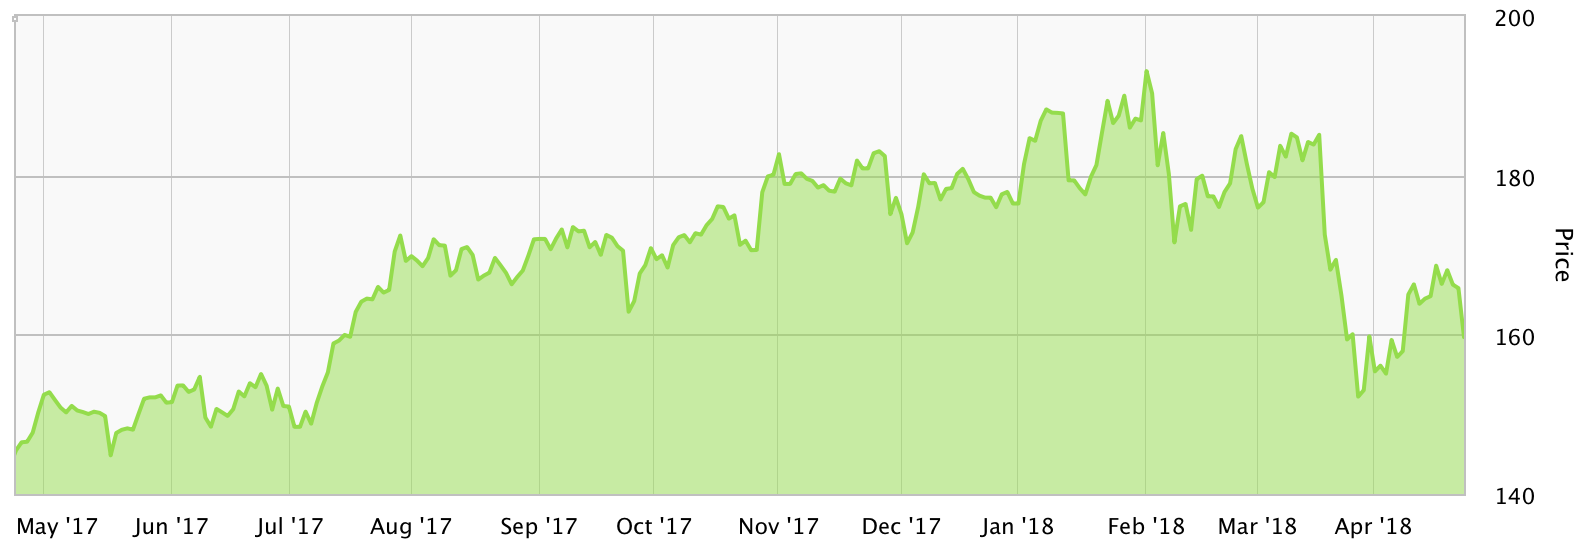
\includegraphics[scale=0.5]{FacebookYear.png}
  \caption{Facebook Stock Price \\
  \small Facebook stock price figure showing drastic decline at the beginning of April}
  \label{fig:faceplant}
\end{figure}

The most prominent feature in Figure \ref{fig:faceplant} is the dramatic drop around the beginning of April. Mark Zuckerburg testified before congress on April 8th. This hearing caused concern about Facebook's future, where traders expected Facebook's stock price to continue declining around a window of April 8th, according to Business Insider [1].

This project will examine the extent to which media sources affect stock prices, and how well media data affects stock price changes.

\newpage 

\section{Methods}

The focus of this project is to investigate the effects of media on stock price changes inside the technology industry. A single industry was chosen in order to maintain consistent results. The companies in this project representing the tech industry are: \\
\\
1. Hewlett Packard \\
2. IBM \\
3. Seagate \\
4. Western Digital \\
5. Intel \\

The main media data is textual data from news articles into our model. The articles were gathered from reputable news sources, such as the Wall Street Journal. 

Furthermore, data from Google Trends is also included to obtain correlation between certain textual features to model public interest in the company.  

Numerical data measuring the closing price and volatility of shares was retrieved from Bloomberg. Other numerical data included macro-economic factors, such as the S\&P500, crude oil, and gold, in order measure a complete market change, as opposed to individual company changes. 

As a baseline model, a simple regression was used to establish a relationship between stock price and google trends. 

In order to begin analyzing text data, a logistic regression was used to model the impact of words on a binary, up-down change in the stock price. As an extention to this, this project team used Topic Modeling to determine different themes occurring within articles. These themes were then futher used in a model to determine effectiveness. Finally, a Recurrent Neural Networks (RNN) was used as a neural network model able to adapt to and store previous article data. 

\newpage
\section{Results and Discussion}

The Google Trends data provided an excellent starting point for this analysis. As one would expect, given that they measure public interest in a company, the Google Trends, when combined with previous stock data, was used in predicting the closing price of the company's shares. 

The Google Trends data combined with previous stock data when predicted the closing price of the company's shares. 

\begin{figure}[H]
	\centering
    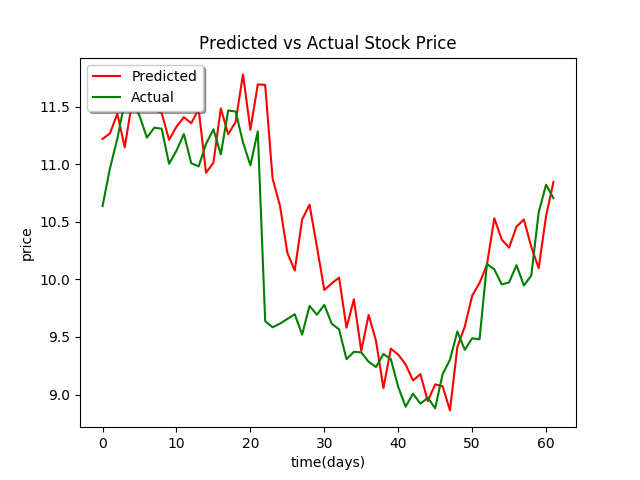
\includegraphics[scale=0.5]{googleHP.png}
  \caption{Prediction Results \\
  \small Graph showing predicted closing stock price versus actual value generated from a basic regression model for HP data}
  \label{fig:googlehp}
\end{figure}
For example, Figure \ref{fig:googlehp} shows almost exact results using a standard regression, where the Predicted and Actual curves are almost completely correlated. 

The following table details Mean Squared Error (MSE) per company. 

Unfortunately, the MSE of the regression model seemed to increase with additional data. This is quite contradictory to standard intuition, where error tends to decrease as the number of features increases. 

\begin{figure}[H]
	\centering
    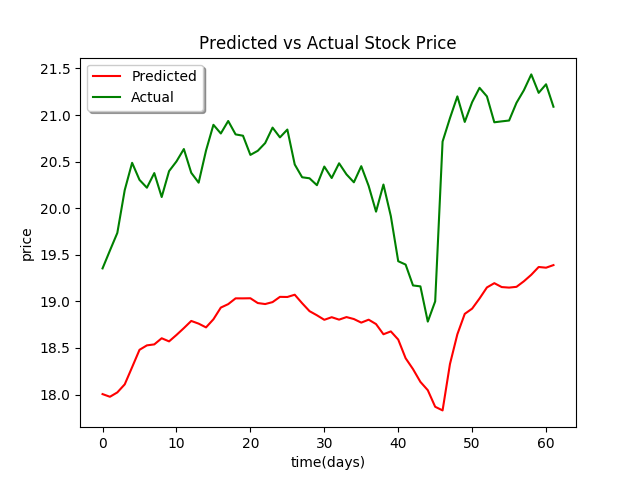
\includegraphics[scale=0.5]{googleIBM.png}
  \caption{Prediction Results \\
  \small Graph, using Google Trends, showing small covariance with large bias / error for IBM data}
  \label{fig:googleibm}
\end{figure}

Figure \ref{fig:googleibm} shows the large error for IBM, possibly as a result of overfitting. Techniques such as regularization and normalization were attempted, but to limited effectiveness. 

\section{Conclusions}

The team was able to flesh out a solid model, with low error rates. This model can easily be built upon to include more data sources, such as twitter and annual legal data. 

One of the biggest challenges was getting enough clean data from a variety of sources. Despite our efforts, there were often significant gaps in dates between published articles.

RNN’s are potentially a great tool for stock predictions, but they require a large amount of data to achieve maximum potential. In a low data situation, a generative model is one of the best choices. However, as more data is collected and the gaps are filled, the RNN will continue to improve and eventually outperform a generative model. 


\section{References}

\small

\subsection{Figures}

Figure \ref{fig:faceplant} from Yahoo Finance

Figure \ref{fig:googlehp} created by Aniq Shahid's tensorflow model. 

\subsection{Citations}

[1] Ciolli, Joe (2018, April 10) \emph{Facebook traders are bracing for the worst ahead of Mark Zuckerberg's hearing}. Retrieved from \url{http://www.businessinsider.com/facebook-stock-price-hedging-ahead-of-mark-zuckerberg-congressional-testimony-hearing-2018-4}

\end{document}
